%% ============================================================================
%% methodology_results_emcee.tex
%%
%% Methodology + Results sections for the emcee-combination track of the current
%% GRB redshift-estimation pipeline. Follow-up to Narendra et al. (A&A
%% aa52651-24corr). Written for the A&A aa.cls document class so it drops into
%% the existing Overleaf project; a minimal title/author stub and an embedded
%% thebibliography are included so it also compiles standalone.
%%
%% NOTE: the linear-z formula rerun (Eq.~\ref{eq:winner}), the baseline
%% SuperLearner results (Sect.~\ref{sec:res-cv}), the donor-matched OT-fusion
%% rerun (Sect.~\ref{sec:ot}), and the augmented SuperLearner rerun
%% (Sect.~\ref{sec:sl}) are all now final on the corrected 266-burst sample;
%% all three are tabulated as current results in Sect.~\ref{sec:res-cv}.
%% ============================================================================
\documentclass{aa}

\usepackage{graphicx}
\usepackage{amsmath}
\usepackage[T1]{fontenc}

% Shorthands for the plateau/prompt symbols, matching the parent paper.
\newcommand{\Fa}{F_a}
\newcommand{\Ta}{T_a}
\newcommand{\NH}{N_{\rm H}}
\newcommand{\logz}{\log_{10}(z+1)}
\newcommand{\grb}[1]{GRB\,#1}

\begin{document}

\title{Extending GRB redshift estimation to optical-plateau bursts:
       methodology and results}
\author{P.~Lin \and collaborators}
\institute{(affiliations)}
\date{Draft \today}

% aa.cls requires an abstract before \maketitle; this stub is for standalone
% compilation only -- delete the title/author/abstract block when pasting the
% two sections into the main manuscript.
\abstract
{Gamma-ray bursts (GRBs) are powerful probes of the distant Universe, but fewer
 than 15\% have a measured redshift, and machine-learning (ML) estimators
 trained on the X-ray afterglow plateau leave out the sizeable population of
 long GRBs (LGRBs) whose plateau is instead measured in the optical band.}
{We extend the ML redshift estimator of \citet{narendra2025} to fold
 optical-plateau LGRBs onto the common X-ray parameter scale, testing whether
 the enlarged, more heterogeneous training sample retains the parent model's
 accuracy, and re-deriving its formula search directly in the linear-redshift
 metric the parent paper itself uses for formula selection.}
{We cross-calibrate the four shared optical/X-ray plateau parameters with an
 \texttt{emcee} MCMC linear regression on 78 dual-catalogue anchor bursts,
 project 83 optical-only bursts onto the X-ray scale by posterior-predictive
 propagation, apply quality and M-estimator robust-regression outlier cuts,
 run a 100-split formula search over the $16{,}510$-formula library of
 \citet{narendra2025} scored in linear redshift space, and train a stacked
 SuperLearner ensemble with Monte Carlo error propagation.}
{After cuts, 266 LGRBs remain for ensemble training. The search selects a
 formula in which $\log T_{90}$, rather than $\log \Ta$, enters the leading
 second-order interaction block, chosen by a difficulty-adjusted vote across
 all 100 splits. The baseline SuperLearner reaches $r=0.672$ in $\logz$ over
 213 cross-validated bursts ($r=0.720$ excluding $2\sigma$ Monte Carlo
 outliers), matching the pure-X-ray-trained parent model despite the added
 optical-domain heterogeneity, and rises to $r=0.964$ for the subset falling
 inside its own $1\sigma$ Monte Carlo interval.}
{Cross-calibrating optical- and X-ray-domain plateau parameters recovers a
 redshift estimator that performs on par with the X-ray-only model while
 extending its reach to bursts without any X-ray afterglow plateau, showing
 that optical-plateau LGRBs are a viable additional pool for future ML
 training samples. Two alternatives to this configuration -- a donor-matched
 optimal-transport-style combination in place of the \texttt{emcee}
 cross-calibration, and an augmented SuperLearner with additional
 domain-adaptation machinery -- both underperform it ($r=0.630$ and $r=0.650$
 respectively, versus $0.720$), indicating the simpler combination and ensemble
 choices are currently the better ones. We also find that reproducing the
 parent paper's single-split diagnostic directly, rather than an aggregate
 across splits, is essential to correctly interpret which formulae the search
 actually favours.}
\keywords{gamma-ray bursts -- methods: statistical -- methods: data analysis}

\maketitle

%% ============================================================================
\section{Introduction}
\label{sec:intro}

Gamma-ray bursts (GRBs) are detected across the full range of observable
redshift and, once standardised, can extend the cosmological distance ladder
well beyond what is reachable with Type~Ia supernovae. Realising this
potential requires a large sample of bursts with known redshift, yet fewer
than 15\% of GRBs currently have one, chiefly because spectroscopic follow-up
demands large-aperture telescope time that is not always available promptly
after the trigger \citep{narendra2025}. The Dainotti relation between the
rest-frame end time of the X-ray afterglow plateau and its luminosity offers
one route around this bottleneck, and a growing body of work has used it,
together with other plateau- and prompt-emission properties, to train ML
models that predict a burst's redshift from its afterglow parameters alone
\citep{narendra2025}. \citet{narendra2025} (itself building on the training
sample of \citealt{dainotti2024c}) trained a stacked SuperLearner ensemble on
238 LGRBs with a Swift/XRT-fitted X-ray plateau, obtained a cross-validated
$r=0.646$ in $\logz$ (rising to $r=0.89$ after an optimal-transport bias
correction), and released pseudo-redshifts for a further 276 LGRBs together
with a public web app.

That model, however, can only be applied to bursts whose X-ray light curve
was well enough sampled to fit a plateau. A comparably sized population of
LGRBs instead has a well-measured \emph{optical} afterglow plateau but no
usable X-ray plateau -- either because the burst was not observed early
enough in X-rays or because ground-based and space telescopes captured the
optical decay in more detail. The plateau feature is not unique to X-rays: an
analogous two- and three-dimensional fundamental-plane correlation has been
established at optical wavelengths for a sample of nearly 180 GRB afterglows
\citep{dainotti2022optical}, and a public catalogue of 536 GRBs with measured
optical afterglow and redshift, of which roughly a third show a plateau, is
now available \citep{dainotti2024a}. This optical-plateau population is
presently unused by X-ray-only ML redshift estimators, even though its
plateau parameters are physically analogous to their X-ray counterparts.

In this work we extend the methodology of \citet{narendra2025} to make use of
this population. Because the optical- and X-ray-domain plateau parameters are
measured in different bands and are only tightly correlated rather than
identical, folding optical-only bursts into the X-ray-trained model requires
an explicit cross-calibration step, for which we use a Bayesian
(\texttt{emcee}) linear regression on the bursts common to both catalogues.
We then re-apply the parent paper's full downstream pipeline -- LASSO feature
selection, formula generation, robust outlier removal, SuperLearner training,
and Monte Carlo error propagation -- to the combined sample, with one
methodological correction: we score the formula search directly in linear
redshift space, matching the axes and cutoffs of the parent paper's own
selection diagnostic (their Fig.~6), rather than in log space only. This
paper is organised as follows. Section~\ref{sec:methodology} describes the
cross-calibration, cuts, and downstream pipeline; Sect.~\ref{sec:results}
presents the resulting formula, SuperLearner performance, and Monte Carlo
calibration; Sect.~\ref{sec:discussion} discusses these results in the
context of \citet{narendra2025} and of near-term multi-band missions; and
Sect.~\ref{sec:conclusions} summarises our conclusions.

%% ============================================================================
\section{Methodology}
\label{sec:methodology}

We build directly on the machine-learning (ML) redshift estimator of
\citet{narendra2025}, which trained a SuperLearner ensemble on the X-ray-plateau
parameters of long gamma-ray bursts (LGRBs). The central extension presented here
is the incorporation of \emph{optical-plateau} LGRBs into the training sample: a
sizeable population of bursts possess a well-measured optical afterglow plateau but
no X-ray plateau, and folding them onto the common X-ray parameter scale enlarges
the labelled sample. Because the optical- and X-ray-domain plateau parameters are
physically distinct but tightly correlated, this requires an explicit
cross-calibration step before the paper's downstream pipeline (feature selection,
formula generation, robust outlier removal, ensemble learning, and Monte Carlo
error propagation) can be applied. Each stage is described below; unless stated
otherwise the response variable is $\logz$ and all logarithms are base 10, following
\citet{narendra2025}.

\subsection{Data samples}
\label{sec:data}

We use two catalogues of LGRBs with spectroscopic redshift. The X-ray sample
contains 223 bursts whose afterglow plateau was fitted in the $0.3$--$10$~keV Swift
XRT band with the \citet{willingale2007} (W07) function, from which we take the four
plateau parameters $\log \Fa$ (plateau end flux), $\log \Ta$ (plateau end time),
$\alpha$ (post-plateau temporal decay index) and $\beta$ (plateau spectral index),
together with the prompt-emission quantities $\log T_{90}$, $\log$~Fluence,
$\log$~PeakFlux, the prompt photon index, the X-ray spectral index $\Gamma$, and the
hydrogen column density $\log \NH$. The optical sample contains 161 LGRBs whose
plateau was instead measured in the optical band, providing optical-domain
counterparts of the same four plateau parameters. Of these, \textbf{78} bursts
(``anchors'') appear in both catalogues and constrain the optical$\rightarrow$X-ray
calibration, while \textbf{83} are optical-only and are the targets of the
projection. The ten candidate features listed above are identical to those of
\citet{narendra2025}; see their Sect.~3 and Fig.~1 for the plateau definition.

Figure~\ref{fig:scattermatrix} compares the two source populations directly, in the
style of Fig.~2 of \citet{narendra2025}, across all ten candidate features plus
redshift, on the 285-burst sample after the long-GRB scope cut but before the
non-negotiable cuts of Sect.~\ref{sec:cuts}. The two populations are broadly
consistent in shape for most features, with the clearest differences in $\log \Fa$
(the optical-sourced bursts skew to somewhat higher values) and in the
$\log \Fa$--$\log \Ta$ anti-correlation, which is stronger for the X-ray-native
subset ($-0.76$) than for the optical-sourced one ($-0.62$); both are consistent in
sign and magnitude with the plateau physics underlying the Dainotti relation.

\begin{figure*}
  \centering
  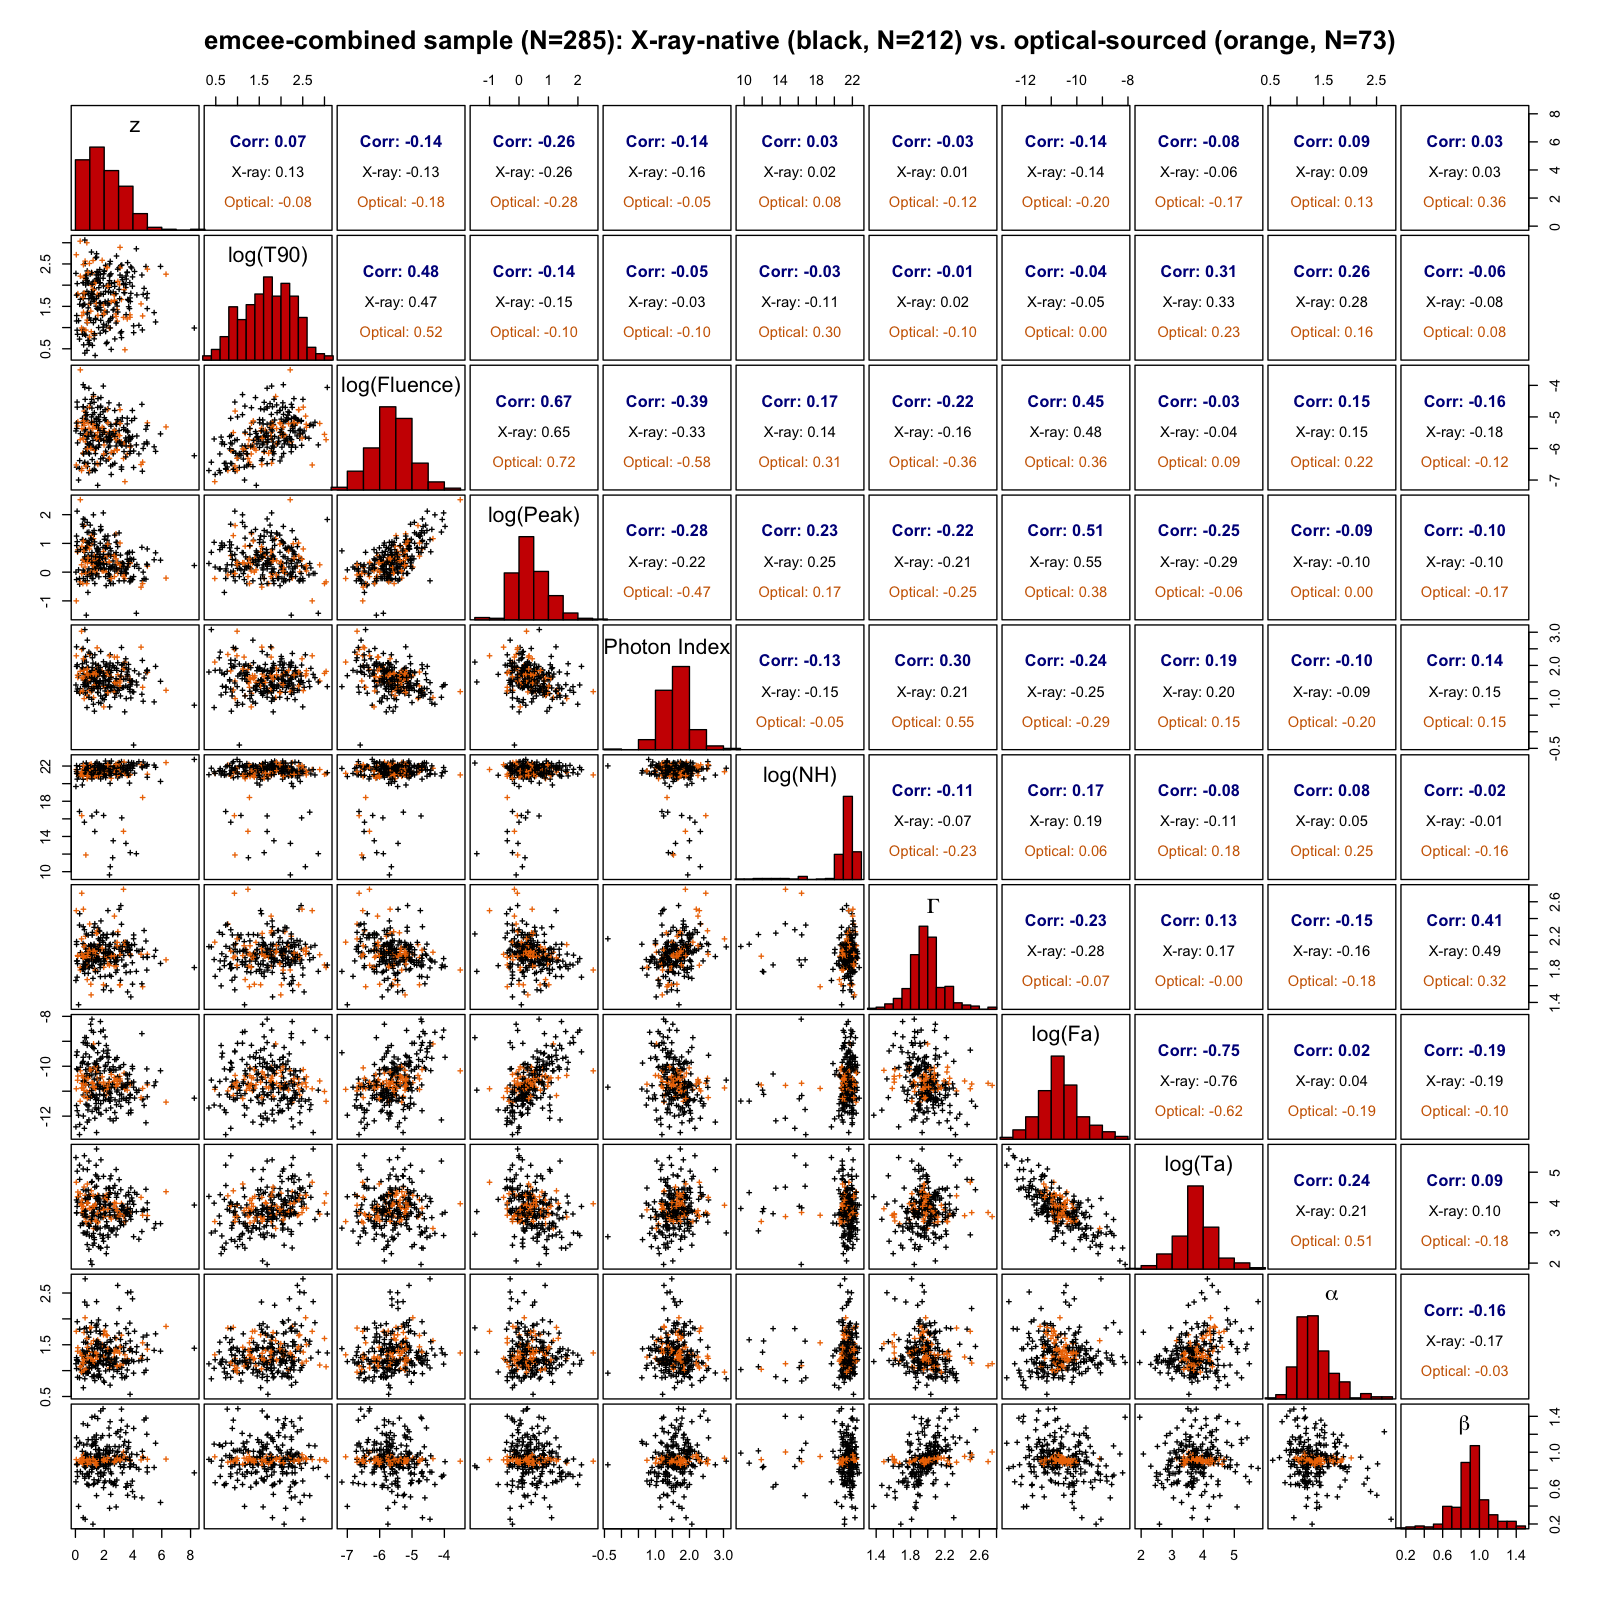
\includegraphics[width=0.95\textwidth]{figures/scatter_matrix_emcee_v2_native_vs_optical.png}
  \caption{Scatter matrix of the ten candidate features plus redshift for the
    285-burst emcee-combined sample (post scope cut, pre non-negotiable cuts),
    split by source population: X-ray-native (black, $N=212$) versus
    optical-sourced (orange, $N=73$). Diagonal: histograms. Lower triangle:
    per-burst scatter. Upper triangle: Pearson correlation coefficients, overall
    (blue) and per population (black/orange).}
  \label{fig:scattermatrix}
\end{figure*}

\subsection{Cross-calibration and catalogue combination}
\label{sec:emcee}

For each of the four shared plateau parameters we fit a linear optical$\rightarrow$
X-ray calibration on the 78 anchors,
\begin{equation}
  y = m\,x + b,
  \label{eq:calib}
\end{equation}
where $x$ and $y$ are the optical- and X-ray-domain values. We treat the reported
$1\sigma$ measurement uncertainties on both axes together with an intrinsic scatter
$s$ through a Gaussian likelihood with total variance
\begin{equation}
  V = \sigma_y^2 + m^2\,\sigma_x^2 + s^2,
  \label{eq:variance}
\end{equation}
sampling the parameters $\theta=(m,b,\ln s)$ with flat priors using the affine-
invariant ensemble sampler \texttt{emcee}. We run 32 walkers for 3000 steps,
discarding the first 500 as burn-in and thinning by 15, and pool \textbf{four}
independently seeded chains per parameter into a single posterior; the point estimate
is the posterior median and the $1\sigma$ error the posterior standard deviation. The
fit is fully deterministic under fixed seeds. The optical-only bursts are then
projected onto the X-ray scale by full posterior-predictive propagation: for every
posterior draw $(m_i,b_i,s_i)$ each optical measurement is perturbed within its
$1\sigma$ error, mapped through Eq.~(\ref{eq:calib}) with an added scatter term, and
summarised by the median (point estimate) and half the 16th--84th percentile range
($1\sigma$). When a burst has both an X-ray and a projected optical value for a given
column, the X-ray measurement is preferred and the projection serves only as a
fallback. The combined catalogue at this stage contains \textbf{306} bursts (223
X-ray plus 83 projected optical-only). Figure~\ref{fig:calib} shows the calibration.

\begin{figure}
  \centering
  
\includegraphics[width=\linewidth]{figures/emcee_optical_vs_xray.png}
  \caption{Optical versus X-ray plateau parameters ($\log \Fa$, $\log \Ta$,
    $\alpha$, $\beta$) on the 78 anchor GRBs, with the \texttt{emcee}
    optical$\rightarrow$X-ray calibration (Eq.~\ref{eq:calib}) overplotted.}
  \label{fig:calib}
\end{figure}

\subsection{Alternative combination: donor-matched fusion}
\label{sec:ot}

As a cross-check on the emcee-based combination above, we built a second,
independent combined catalogue using a donor-matched fusion approach. The two
combinations share their treatment of the four calibrated plateau parameters
($\log \Fa$, $\log \Ta$, $\alpha$, $\beta$): the fusion approach reuses the same
cached \texttt{emcee} posterior of Eq.~(\ref{eq:calib}) rather than fitting its own
calibration, so any difference between the two combined catalogues is confined to
how the remaining, non-plateau features are filled in for the 83 optical-only
bursts. $\log T_{90}$ is taken directly from the optical catalogue's own
measurement in both combinations, as it is a directly observed quantity in either
band. The other five ($\gamma$, photon index, $\log \NH$, $\log$~Fluence,
$\log$~PeakFlux) have no X-ray-band measurement at all for optical-only bursts, and
it is only these five that the two combinations fill in differently.

Rather than a single population-level imputation, each optical-only burst is
matched against the 223 X-ray-native donors by distance in the (weighted,
standardised) four-dimensional plateau-parameter space, using a Gibbs/softmax
kernel, $w_i \propto \exp(-d_i/h)$, normalised per query burst ($d_i$ the
weighted distance to donor $i$; $h$ a bandwidth selected by leave-one-out
cross-validation on the 78 anchors, treated as if they were optical-only). The
imputed value is the donor-weighted mean of each target feature, and the
donor-weighted spread around that mean supplies a native, per-burst uncertainty
estimate -- a diffuse match yields a large uncertainty, a tight match a small one
-- so no separate uncertainty model is needed for these five features. An earlier,
balanced-optimal-transport (Sinkhorn) version of this matching over-smoothed and
is superseded by the kernel form above; we retain the name ``fusion'' from that
lineage.

The leave-one-out check also validates the method directly: for each of the 78
anchors in turn, we withhold its real X-ray-measured value for the five features
and re-derive it from the other 222 donors. Recovery is weak to moderate
(Table~\ref{tab:otloo}) -- expected, since these five features are only weakly
correlated with the plateau parameters used for matching (Fig.~\ref{fig:scattermatrix}
shows this directly) -- but the per-burst uncertainty is reasonably well calibrated:
the true value falls within $\pm1$ donor-weighted$\sigma$ for $55$--$67\%$ of anchors
on four of the five features, close to the nominal $68\%$ for a correctly sized
$1\sigma$ interval.

\begin{table}
  \centering
  \caption{Leave-one-out validation of the donor-matched fusion imputation on the
    78 anchor GRBs: Pearson correlation and RMSE between each anchor's true,
    withheld X-ray value and its value re-derived from the other 222 donors, and
    the fraction of anchors whose true value falls within $\pm1$ donor-weighted
    $\sigma$ of the re-derived value.}
  \label{tab:otloo}
  \begin{tabular}{lccc}
    \hline\hline
    Feature & $r$ & RMSE & $1\sigma$ coverage \\
    \hline
    $\gamma$            & 0.06 & 0.15 & 55\% \\
    Photon index        & 0.12 & 0.41 & 67\% \\
    $\log \NH$          & 0.09 & 2.02 & 92\% \\
    $\log$~Fluence      & 0.31 & 0.57 & 58\% \\
    $\log$~PeakFlux     & 0.29 & 0.51 & 59\% \\
    \hline
  \end{tabular}
\end{table}

Applying the same non-negotiable cuts of Sect.~\ref{sec:cuts} to this
donor-matched catalogue flags the identical four bursts as the emcee combination
(Sect.~\ref{sec:emcee}), 285$\rightarrow$281, and the same downstream pipeline
(Sects.~\ref{sec:lasso}--\ref{sec:mc}) has now been re-run on it under the same
linear-$z$ formula search; its winning formula, M-estimator cut, and baseline
SuperLearner performance are reported alongside the emcee-based results in
Sect.~\ref{sec:res-cv}.

\subsection{Quality and non-negotiable outlier cuts}
\label{sec:cuts}

Two cuts precede feature selection. First, at the combination stage we remove any
optical-only burst whose relative error $|\sigma|/|{\rm value}|$ exceeds $0.5$ on any
of the four calibrated parameters, on either the original-optical or the projected-
X-ray side; this reduces the sample to \textbf{296}. Second, we apply a set of
non-negotiable physical cuts. We restrict to long bursts via $\log T_{90} > \log 2$
(285 bursts remain) and then remove bursts with unphysical parameter values
($\alpha>3$, $\beta>2$, $\log T_{90}>6$, or a negative photon index), together with a
relative-error cut $|\sigma|/|{\rm value}|>0.5$ that is deliberately restricted to
the four \emph{fitted} plateau parameters ($\alpha$, $\beta$, $\log \Fa$,
$\log \Ta$). We do not apply this error cut to the directly measured catalogue
quantities ($T_{90}$, photon index, fluence, $\NH$, peak flux): a large relative
error there reflects genuine measurement noise rather than an unreliable calibration
fit, and cutting on it would preferentially discard faint, high-redshift bursts. This
stage flags four bursts --- \grb{090516A}, \grb{100621A}, \grb{131117A}, and
\grb{230328B} --- leaving \textbf{281} bursts for training. The same counts and the
same four flagged bursts are obtained independently for the alternative
donor-matched fusion combination of Sect.~\ref{sec:ot}. Table~\ref{tab:outliers}
lists these four bursts together with the fifteen removed at the M-estimator
stage below (Sect.~\ref{sec:mest}).

\begin{figure}
  \centering
  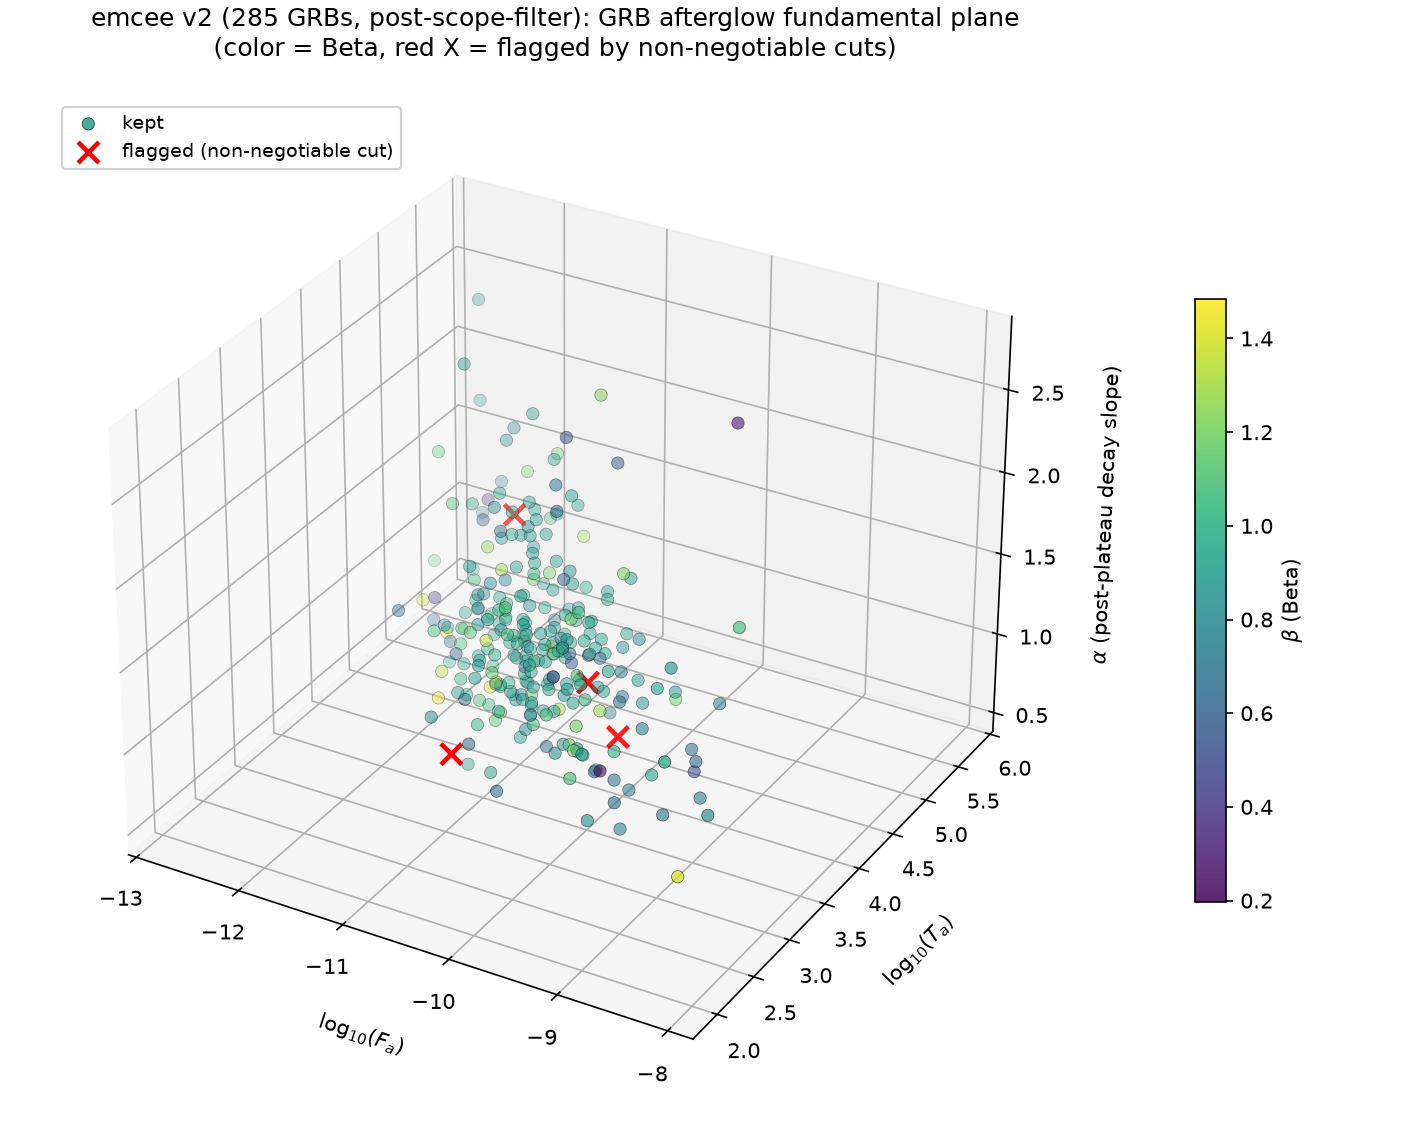
\includegraphics[width=\linewidth]{figures/fundamental_plane_4d_emcee_v2_current.png}
  \caption{The plateau fundamental plane ($\log \Fa$, $\log \Ta$, $\alpha$; colour
    $=\beta$) for the 285-burst emcee-combined sample, with the four bursts flagged
    by the non-negotiable cuts of this section marked with a red $\times$.}
  \label{fig:4d}
\end{figure}

\subsection{Feature selection}
\label{sec:lasso}

Following \citet[Sect.~4.2.1]{narendra2025} we rank the ten candidate features with
the least absolute shrinkage and selection operator \citep[LASSO;][]{tibshirani1996}.
We run \texttt{cv.glmnet} ($\alpha=1$) 100 times, each time recording the coefficient
vector at $\lambda_{\rm 1se}$, average the 100 vectors, and order the features by
mean absolute coefficient. The seven highest-ranked features are retained:
$\log \NH$, $\log$~PeakFlux, photon index, $\log \Ta$, $\log \Fa$, $\log T_{90}$, and
$\alpha$ (Fig.~\ref{fig:lasso}), matching the seven-feature choice of the parent
paper. This ranking selects the features used to build the formula library of
Sect.~\ref{sec:formula}; the SuperLearner ensemble of Sect.~\ref{sec:sl} performs
its own, separate invocation of the same LASSO procedure and does not restrict it
to seven features.

\begin{figure}
  \centering
  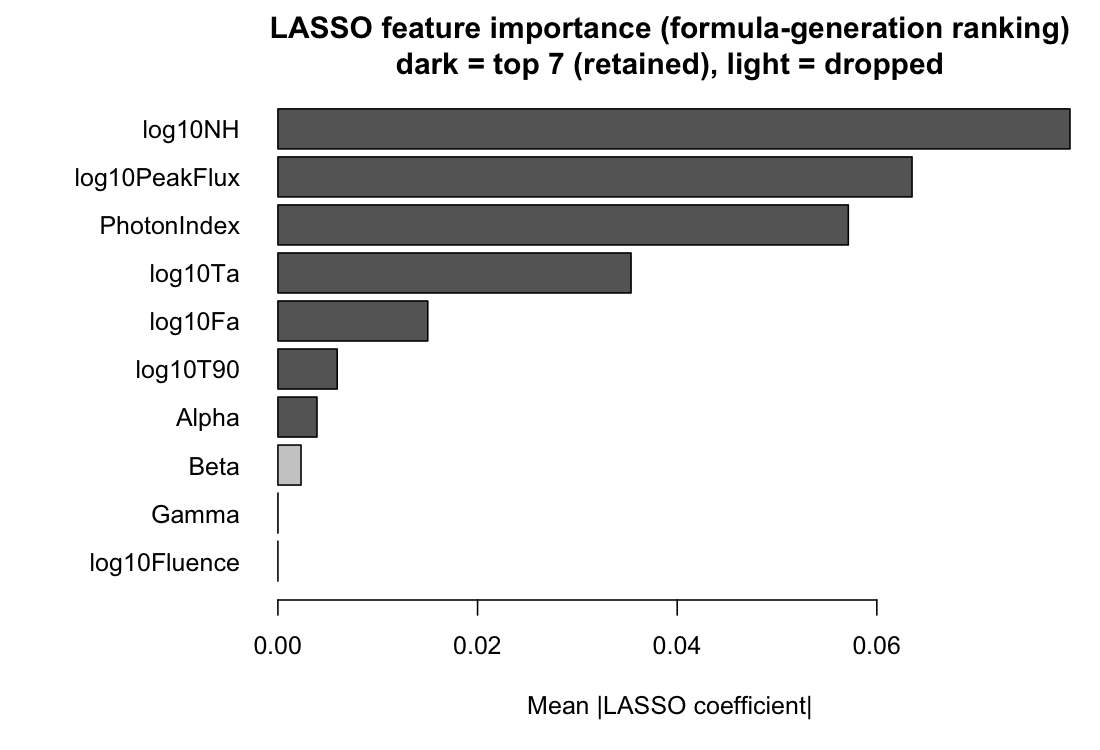
\includegraphics[width=\linewidth]{figures/LassoFeatures_formulagen.png}
  \caption{Mean absolute LASSO coefficient of each candidate feature over 100
    resamples, from the invocation that selects the formula library's seven
    features (dark bars retained, light bars dropped).}
  \label{fig:lasso}
\end{figure}

\subsection{Formula generation and selection}
\label{sec:formula}

From the seven selected features and their seven squared terms we generate the
formula library of \citet[Sect.~4.2.3]{narendra2025}. The second-order (O2) library
enumerates every non-empty subset of the 14 linear-plus-squared terms, wrapped in a
pairwise-interaction operator, giving $2^{14}-1 = \mathbf{16{,}383}$ formulae; the
linear-only (O1) library gives $2^{7}-1 = \mathbf{127}$; a further \textbf{148}
smoothed-term (GAM) formulae are generated separately. The total of
$127+16{,}383=\mathbf{16{,}510}$ matches the count reported by \citet{narendra2025}.
The search operates on the O2 library.

Each formula is evaluated over \textbf{100} randomised $80{:}20$ train/test splits.
Within a split, every formula receives a ten-fold cross-validation (10fCV) pass on
the training set, and its correlation $r$ and RMSE are computed in \emph{linear}
redshift space (predictions are transformed $z = 10^{\rm pred}-1$ before scoring), so
that the selection metrics correspond to the linear axes of Fig.~6 of
\citet{narendra2025} and their cutoffs ($r=0.565$, ${\rm RMSE}=1.167$). Formulae with
$r$ above the $99.9$th percentile \emph{and} RMSE below the 2nd percentile of the
split are carried to the held-out test set. On the test set we additionally compute
the bias $\langle z_{\rm pred}-z_{\rm obs}\rangle$ and use it as a \emph{gate}: the
worse half by $|{\rm bias}|$ is discarded, after which the best-$r$ and best-RMSE
survivors each cast one vote. We adopt bias as a gate rather than an equal-weight
vote because the single-split best-$|{\rm bias}|$ formula scatters across nearly all
100 splits, indicating that the mean signed residual of one split is too noisy to
vote on directly. Across the 100 splits (200 votes cast: one best-$r$ and one best-RMSE per split
among the bias-gated survivors, spread over 95 distinct formulae) the most-voted
formula, with 8 votes, is
\begin{align}
  \logz \sim\; &(\log \Fa^2 + \log T_{90} + \log \Fa + \log{\rm PeakFlux})^2 \nonumber\\
       &+ \log \NH + {\rm PhotonIndex} + \log \Ta + \alpha \nonumber\\
       &+ \log \NH^2 + \log{\rm PeakFlux}^2 + {\rm PhotonIndex}^2 \nonumber\\
       &+ \log \Ta^2 + \log T_{90}^2 + \alpha^2 .
  \label{eq:winner}
\end{align}
Notably $\log T_{90}$ enters the core interaction block in place of $\log \Ta$,
which is retained only as an additive term -- a structurally different formula
from every earlier (log-space-scored) iteration of this search, reflecting the
switch to linear-$z$ scoring. The search is checkpointed after every split and is
fully resumable. Figure~\ref{fig:formula} reproduces Fig.~6 of
\citet{narendra2025} directly for one representative split: the full library with
the threshold-surviving candidates marked (left) and those candidates' held-out
test performance (right), with the overall winning formula highlighted where it
appears as a candidate.

\begin{figure}
  \centering
  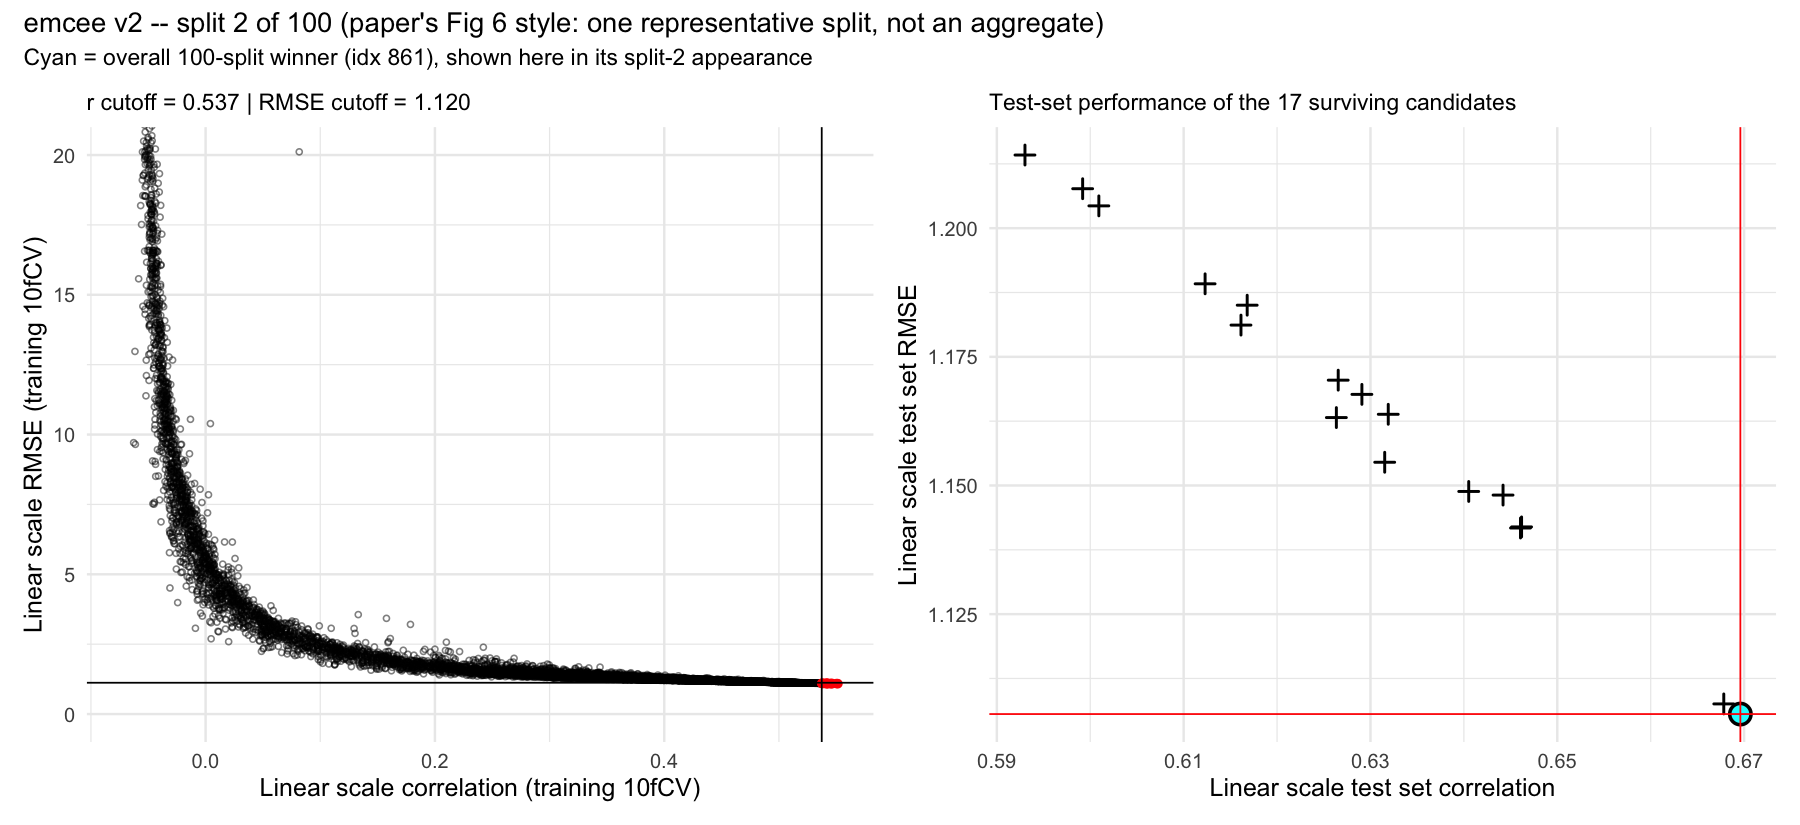
\includegraphics[width=\linewidth]{figures/fig6_paper_style_emcee_LINEARZ_run.png}
  \caption{Reproduction of Fig.~6 of \citet{narendra2025} for a single
    representative split (of 100): linear-scale RMSE versus correlation for the
    full 16{,}383-formula library (left, red = surviving the training-CV
    threshold) and the held-out test-set performance of those survivors (right,
    highlighted = overall winning formula, Eq.~\ref{eq:winner}). This is a
    per-split illustration, not an aggregate across splits -- a formula's
    apparent performance in any single split reflects that split's own
    difficulty as well as the formula itself, which is why the search tallies
    votes across all 100 splits (Sect.~\ref{sec:res-formula}) rather than
    ranking formulae by any single split's numbers.}
  \label{fig:formula}
\end{figure}

\subsection{Robust removal of catastrophic outliers}
\label{sec:mest}

Before ensemble training we apply the M-estimator cut of
\citet[Sect.~4.3]{narendra2025}. A Huber robust regression (\texttt{MASS::rlm},
method \texttt{M}) is fitted with the winning formula (Eq.~\ref{eq:winner}), and the
bursts in the lowest $5\%$ of robustness weight are removed. This flags
\textbf{15} of the \textbf{281} bursts (robustness weight $\leq0.6098$), leaving
\textbf{266} bursts for ensemble training.

\begin{table}
  \centering
  \caption{All 19 bursts removed from the 285-burst emcee-combined sample before
    ensemble training: four by the non-negotiable cuts of Sect.~\ref{sec:cuts}
    (reason given) and fifteen by the M-estimator cut of this section (robustness
    weight given; threshold $\leq0.6098$), ordered by increasing weight.}
  \label{tab:outliers}
  \begin{tabular}{ll}
    \hline\hline
    GRB & Reason / weight \\
    \hline
    \multicolumn{2}{l}{\emph{Non-negotiable cuts (Sect.~\ref{sec:cuts})}} \\
    \grb{090516A} & err$>$value: $\beta$ \\
    \grb{100621A} & err$>$value: $\beta$ \\
    \grb{131117A} & photon index $<0$ \\
    \grb{230328B} & err$>$value: $\beta$ \\
    \hline
    \multicolumn{2}{l}{\emph{M-estimator cut (this section), weight $\leq0.6098$}} \\
    \grb{051109B} & 0.373 \\
    \grb{050826A} & 0.427 \\
    \grb{100508A} & 0.490 \\
    \grb{070809A} & 0.495 \\
    \grb{160314A} & 0.546 \\
    \grb{130606A} & 0.551 \\
    \grb{220521A} & 0.572 \\
    \grb{220101A} & 0.582 \\
    \grb{070714B} & 0.587 \\
    \grb{161129A} & 0.587 \\
    \grb{080916A} & 0.590 \\
    \grb{100316D} & 0.595 \\
    \grb{111008A} & 0.607 \\
    \grb{101225A} & 0.608 \\
    \grb{060614A} & 0.610 \\
    \hline
  \end{tabular}
\end{table}

\subsection{The SuperLearner ensemble}
\label{sec:sl}

We train the stacked SuperLearner ensemble of \citet[Sect.~4.4]{narendra2025} in two
configurations. Both share the same underlying design matrix for their
general-purpose learners: alongside the GAM/GLM/Bayesian-GLM learners built from
the fixed winning formula (Eq.~\ref{eq:winner}, restricted to its seven features),
the ensemble's remaining learners see a separate, independent invocation of the
LASSO ranking of Sect.~\ref{sec:lasso} (its own 100-repeat \texttt{cv.glmnet}
average, run on this stage's own imputed data) used \emph{unrestricted} -- over all
ten candidate features rather than cut to seven -- together with their squared
terms. Domain membership is further encoded through a Daum\'e-style augmentation
\citep{daume2007}: an \texttt{is\_optical} indicator plus a scaled per-domain copy
of each of the ten features ($c=0.25$), letting penalized/linear learners fit a
shrunk, domain-specific deviation rather than sharing one global slope across both
domains. This is a real, active part of the results reported below, not merely a
planned feature -- it is present whenever the input catalogue carries an
\texttt{is\_optical} column, which the corrected combined catalogue does.

The \emph{baseline} configuration trains this full design (ten features, their
squares, \texttt{is\_optical}, and its ten domain-interaction columns) through a
broad learner library (elastic net, gradient-boosted trees, CART, MARS, bagged
trees, neural network, random forests, stepwise regressions, plus the
formula-restricted GAM/GLM/Bayesian-GLM learners above), imputes missing values
with multiple imputation by chained equations \citep[MICE;][]{vanbuuren2011} using
the predictive-mean-matching ``midastouch'' method with $m=20$ (predictors and
errors imputed separately), stacks by non-negative least squares, and is
cross-validated with 10fCV repeated 10 times.

The \emph{augmented} configuration builds on this same baseline design and adds
several further components aimed at exploiting the optical/X-ray heterogeneity
beyond the shared Daum\'e terms above. Missing predictors are instead co-imputed
with \texttt{missForest} \citep{stekhoven2012missforest} jointly with an unlabelled
generalisation pool (which never sees the redshift). The learner library
additionally includes a band-interaction GLM (with \texttt{is\_optical}
interacting specifically with the four plateau terms) and a boosted additive model
(\texttt{mboost::gamboost}), and stacking is performed with a non-negative ridge
variant of the NNLS meta-learner. A leakage-safe isolation feature (the distance to
each burst's tenth nearest neighbour in standardised predictor space, fitted on
training folds only) supplies an outlier signal to the ensemble.

\paragraph{Real-value recovery.} Two distinct mechanisms exploit the optical
catalogue's own measurements for the 83 optical-only bursts, rather than treating
their non-plateau features as simply missing. First, $\log T_{90}$,
$\log$~Fluence, photon index, $\log \NH$, $\log$~PeakFlux, and $\gamma$ are not
imputed at all for these bursts: since the optical catalogue already carries direct
measurements of them, we substitute those real values in place of a population-level
placeholder. Second, for the four plateau parameters ($\log \Fa$, $\log \Ta$,
$\alpha$, $\beta$), rather than using the single posterior-median projection of
Sect.~\ref{sec:emcee}, we redraw the projection from four different samples of the
\texttt{emcee} posterior $(m,b)$ per optical-only burst, each combined with three
independent \texttt{missForest} imputation seeds (12 frames total), and average the
resulting predictions. This propagates uncertainty in the optical$\rightarrow$X-ray
\emph{calibration itself} through the ensemble, on top of the usual per-burst
measurement-error propagation of Sect.~\ref{sec:mc}, which only the augmented
configuration currently implements.

\subsection{Monte Carlo error propagation}
\label{sec:mc}

We propagate the input measurement uncertainties through the trained ensemble as in
\citet[Sect.~4.7]{narendra2025}. Each mapped feature is perturbed by drawing from
$\mathcal{N}(\mathrm{value}, \sigma_{\rm catalog})$ with $\sigma_{\rm catalog}$
treated as a $1\sigma$ standard deviation, the corresponding squared terms are
regenerated, and $100$ realisations are pushed through the ensemble. For each burst
we report the median prediction, the $68\%$ (``$1\sigma$'') interval, and whether the
true $\logz$ lies inside that interval (``inside the cone''). Throughout, the metrics
follow the parent paper: the correlation $r$, RMSE, bias, and the normalised median
absolute deviation ${\rm NMAD}=\mathrm{median}\,|\Delta z/(1+z_{\rm obs})|$, together
with the $1\sigma$/$2\sigma$ cone half-widths defined from the standard deviation of
the log-scale residual $\Delta\logz$.

%% ============================================================================
\section{Results}
\label{sec:results}

The formula search now scores in linear-$z$ space (Sect.~\ref{sec:formula}) and the
non-negotiable and M-estimator cuts have converged to their final counts
(Sects.~\ref{sec:cuts}, \ref{sec:mest}); the numbers below are final on the
corrected 266-burst sample, for all three configurations now run on it: the
baseline SuperLearner on the emcee combination (our headline result), the same
baseline on the donor-matched OT-fusion combination of Sect.~\ref{sec:ot}, and
the augmented SuperLearner (Sect.~\ref{sec:sl}) on the emcee combination.

\subsection{Cross-validated redshift estimation}
\label{sec:res-cv}

Table~\ref{tab:cv} summarises the cross-validated performance of the baseline
SuperLearner configuration on the corrected emcee-combined sample. Over the full
$N=213$ cross-validated bursts the ensemble reaches $r=0.672$ in $\logz$
(RMSE~$=0.134$; $r=0.664$, RMSE~$=0.99$ in linear $z$), coinciding with the headline
correlation of \citet{narendra2025} despite the enlarged and more heterogeneous
training sample. Excluding the nine bursts falling outside their $2\sigma$ Monte
Carlo cone ($N=204$) raises this to $r=0.720$ in $\logz$ (RMSE~$=0.121$; $r=0.70$,
RMSE~$=0.94$ in linear $z$). Figures~\ref{fig:corr-plain} and~\ref{fig:corr-plain-z}
show the predicted-versus-observed relation on the log and linear redshift scales,
respectively.

\begin{table}
  \centering
  \caption{Cross-validated redshift-estimation metrics for the baseline SuperLearner
    configuration on the corrected (266-burst) emcee-combined sample. ``All'' is
    the full cross-validated sample; ``without $2\sigma$ outliers'' excludes bursts
    falling outside their $2\sigma$ Monte Carlo cone; ``inside $1\sigma$ cone'' is
    the subset whose true redshift falls within its $1\sigma$ Monte Carlo interval.}
  \label{tab:cv}
  \begin{tabular}{lccccc}
    \hline\hline
    Subset & $N$ & $r_{\log}$ & RMSE$_{\log}$ & $r_z$ & RMSE$_z$ \\
    \hline
    All                       & 213 & 0.672 & 0.134 & 0.664 & 0.99  \\
    Without $2\sigma$ outliers & 204 & 0.720 & 0.121 & 0.70  & 0.94  \\
    Inside $1\sigma$ cone      & 55  & 0.964 & 0.036 & 0.967 & 0.245 \\
    \hline
  \end{tabular}
\end{table}

\begin{figure}
  \centering
  
\includegraphics[width=\linewidth]{figures/z_pred_v_obs_log_without_catOutl_correlation_plot.png}
  \caption{Predicted versus observed $\logz$ for the baseline SuperLearner
    configuration on the corrected sample, $2\sigma$ Monte Carlo outliers removed
    ($N=204$).}
  \label{fig:corr-plain}
\end{figure}

\begin{figure}
  \centering
  
\includegraphics[width=\linewidth]{figures/z_pred_v_obs_linear_without_catOutl_correlation_plot.png}
  \caption{As Fig.~\ref{fig:corr-plain}, but predicted versus observed on the
    linear redshift scale ($r=0.70$, RMSE~$=0.94$, bias~$=0.20$, NMAD~$=1.23$;
    $N=204$).}
  \label{fig:corr-plain-z}
\end{figure}

Table~\ref{tab:cv-compare} compares this winning configuration against the same
baseline SuperLearner trained instead on the donor-matched OT-fusion combination
of Sect.~\ref{sec:ot}, and against the augmented SuperLearner configuration of
Sect.~\ref{sec:sl} trained on the same emcee combination. Both alternatives are
run end to end on the corrected 266-burst (or, for OT, its own independently
M-estimator-cut) sample, with their own winning formula and cuts where
applicable, not merely re-scored with the emcee formula.

\begin{table}
  \centering
  \caption{Cross-validated redshift-estimation metrics for the two alternative
    configurations, on their own corrected samples: the baseline SuperLearner
    trained on the OT-fusion combination (Sect.~\ref{sec:ot}) instead of the
    emcee combination, and the augmented SuperLearner configuration
    (Sect.~\ref{sec:sl}) trained on the emcee combination. Compare against
    Table~\ref{tab:cv}'s emcee+baseline result, the best of the three.}
  \label{tab:cv-compare}
  \begin{tabular}{lccccc}
    \hline\hline
    Configuration & Subset & $N$ & $r_{\log}$ & RMSE$_{\log}$ & $r_z$ \\
    \hline
    OT + baseline       & All                       & 213 & 0.595 & 0.141 & 0.619 \\
    OT + baseline       & Without $2\sigma$ outliers & 208 & 0.630 & 0.133 & 0.642 \\
    emcee + augmented   & All                       & 192 & 0.629 & 0.133 & 0.655 \\
    emcee + augmented   & Without $2\sigma$ outliers & 189 & 0.650 & 0.129 & 0.673 \\
    \hline
  \end{tabular}
\end{table}

Both alternatives sit consistently below the emcee+baseline result (Table~\ref{tab:cv}:
$r_{\log}=0.720$, $N=204$, ``without $2\sigma$ outliers'') at the comparable
subset: OT+baseline reaches $r_{\log}=0.630$ ($N=208$), and emcee+augmented reaches
$r_{\log}=0.650$ ($N=189$), each roughly 0.07--0.09 below. Neither the alternative
combination method nor the additional SuperLearner machinery (missForest
co-imputation, the band-interaction and boosted-additive learners, alternative
stacking) improves on the simpler emcee+baseline configuration, which is why we
report it as the headline result throughout this paper. We discuss possible
reasons for this in Sect.~\ref{sec:discussion}.

\subsection{Formula-search outcome}
\label{sec:res-formula}

Over the 100 splits the search cast 200 votes (one best-$r$ and one best-RMSE per
split among the bias-gated survivors) across 95 distinct formulae. The winning
formula (Eq.~\ref{eq:winner}) received 8 votes, the most of any formula, and is the
formula used to train the ensemble above and to apply the M-estimator cut of
Sect.~\ref{sec:mest}. We rank formulae by this cross-split vote tally rather than by
any single split's (or any cross-split average's) $r$ or RMSE, because a formula's
apparent standing in one split reflects that split's own difficulty as much as the
formula itself (Sect.~\ref{sec:formula}, Fig.~\ref{fig:formula}); the vote count is
the only comparison that is fair across formulae qualifying as candidates in
different splits.

\subsection{Monte Carlo calibration}
\label{sec:res-mc}

Within the subset of bursts whose true redshift falls inside its own propagated
$1\sigma$ Monte Carlo interval ($N=55$, Sect.~\ref{sec:mc}), the correlation rises
sharply to $r=0.964$ in $\logz$ (RMSE~$=0.036$; $r=0.967$, RMSE~$=0.245$ in linear
$z$), demonstrating that where the input measurement errors are well controlled the
ensemble is strongly predictive (Fig.~\ref{fig:mc}). This subset comprises only
$25.8\%$ of the 213 cross-validated bursts, well under the nominal $68\%$ target for
a $1\sigma$ interval (by contrast, the nominal $2\sigma$ interval contains $96\%$ of
bursts, close to its target), indicating that the propagated $1\sigma$ intervals are
under-dispersed; recalibrating them is left to future work.

\begin{figure}
  \centering
  
\includegraphics[width=\linewidth]{figures/mc_pred_vs_obs_log10_inside.png}
  \caption{Monte Carlo predicted versus observed $\logz$ for the baseline
    configuration, restricted to bursts inside their own $1\sigma$ interval, with
    per-burst $1\sigma$ error bars.}
  \label{fig:mc}
\end{figure}

%% ============================================================================
\section{Discussion}
\label{sec:discussion}

The central result of this work is that folding optical-plateau LGRBs onto the
X-ray parameter scale does not cost accuracy: the baseline SuperLearner's
$r=0.672$ in $\logz$ (Sect.~\ref{sec:res-cv}) matches the $r=0.646$ that
\citet{narendra2025} obtained from a purely X-ray-trained sample, even though
our combined sample is more heterogeneous (it mixes directly measured X-ray
parameters with posterior-predictive optical$\rightarrow$X-ray projections)
and was cut down further by the M-estimator step (266 of 281 bursts, versus
their 5\% cut on 238). This suggests that the emcee cross-calibration of
Sect.~\ref{sec:emcee} propagates optical-domain information onto the X-ray
scale without introducing enough additional scatter to offset the benefit of
the larger sample, at least at the current sample sizes.

The winning formula (Eq.~\ref{eq:winner}) is structurally different from the
formula selected on the pure X-ray sample: $\log T_{90}$ now enters the core
second-order interaction block in place of $\log \Ta$, which is retained only
as a linear additive term. \citet{narendra2025} found $\log \NH$ and
$\log \Ta$ to be, respectively, the first- and second-most predictive
features by LASSO coefficient (their Sect.~5.2); we do not find that
$\log \Ta$'s demotion in the winning formula changes its LASSO ranking
(Sect.~\ref{sec:lasso}), so the effect is specific to the formula search
rather than to feature selection. Two changes could plausibly drive it: the
altered $T_{90}$ distribution introduced by the optical-only bursts, and the
switch to linear-$z$ scoring, which reweights the search toward formulae that
control large linear-scale residuals rather than large log-scale residuals.
Disentangling the two would require rerunning the search in log space on the
combined sample, which we leave to future work.

The Monte Carlo intervals remain under-dispersed: only 25.8\% of bursts fall
inside their nominal $1\sigma$ interval (Sect.~\ref{sec:res-mc}), a very
similar degree of under-dispersion to the $26.9\%$/$24.5\%$ that
\citet{narendra2025} reported for their two configurations despite the
substantially different training sample and formula. That the same qualitative
miscalibration persists across two independently trained pipelines suggests it
is a structural property of the perturb-and-repredict Monte Carlo methodology
of Sect.~\ref{sec:mc} (inherited unchanged from \citealt{narendra2025}) rather
than an artefact of either specific sample, and recalibrating the propagated
intervals -- for example by inflating them to match empirical coverage -- is a
shared open item for both works.

The augmented SuperLearner configuration, now rerun on the corrected sample
(Table~\ref{tab:cv-compare}), reaches $r_{\log}=0.650$ ($N=189$, without $2\sigma$
outliers) against the baseline's $r_{\log}=0.720$ ($N=204$) -- its additional
machinery beyond the baseline's own shared Daum\'e-style domain terms
(missForest co-imputation, the band-interaction and boosted-additive learners,
alternative stacking) not only fails to improve on the baseline but costs some
accuracy. This null (if not negative) result is consistent with
\citet{narendra2025}'s own observation that, even with their enlarged sample,
the available LGRB training set remains at least an order of magnitude
smaller than what more complex learners such as neural networks typically
require: added architectural complexity is unlikely to help until the
training sample itself grows substantially, which is precisely the gap the
optical-plateau population is positioned to fill. The smaller $N$ throughout
(189 versus 204) also reflects the augmented configuration's own, independently
computed $2\sigma$ Monte Carlo cone, which flags more bursts as outliers than the
baseline's; whether that reflects a genuinely wider spread in its predictions or
a difference in how the two configurations' Monte Carlo draws interact with the
missForest/projection-draw imputation of Sect.~\ref{sec:sl} is not yet clear.

The donor-matched OT-fusion combination, run through the same baseline
SuperLearner and its own independent formula search and M-estimator cut, reaches
$r_{\log}=0.630$ ($N=208$, without $2\sigma$ outliers) -- also below the emcee
combination's $0.720$, though by less than the augmented configuration falls
short. Sect.~\ref{sec:ot}'s own leave-one-out validation already showed the
donor-matched imputation recovers the five non-plateau features only weakly to
moderately ($r=0.06$--$0.31$); it is plausible that this comparatively noisier
treatment of those features, relative to the emcee combination's use of the
optical catalogue's own directly measured values for them, is what costs the OT
combination some accuracy downstream, though we have not isolated this from
other differences between the two combinations (e.g.\ each has its own
independently selected winning formula). We note, however, that the two
combinations' M-estimator cuts agree substantially on which specific bursts are
catastrophic outliers -- ten of the fifteen flagged by each combination are the
same bursts -- which is reassuring evidence that both combinations are picking
up on genuine problem bursts rather than combination-specific artefacts.

A methodological point from Sect.~\ref{sec:res-formula} is worth stating
explicitly, since it could otherwise mislead a future extension of this
pipeline: a formula's $r$ or RMSE in any single split, or even its average
across the (non-overlapping) splits in which it happens to survive the
training-CV cut, is not a fair basis for ranking formulae, because different
splits present different intrinsic difficulty ceilings. The cross-split vote
tally used here is difficulty-adjusted by construction and is the metric that
should be extended, rather than any per-split or averaged $r$/RMSE, if the
search is scaled to a larger formula library or sample in the future.

Looking ahead, the population of GRBs with a simultaneously observed optical
and X-ray afterglow is growing. The SVOM mission, operational since its
scientific validation phase concluded in early 2025, detected 86 GRBs in its
first 9.3~months, with roughly three-quarters also seen by other facilities
and the remainder unique to SVOM \citep{daigne2026}; SVOM's rapid-slew,
multi-band design (Sect.~5.6 of \citealt{narendra2025}) makes it a natural
target for the cross-calibration approach developed here, since bursts it
observes simultaneously in the optical and X-ray bands no longer need the
emcee projection step at all and can instead be used to directly test and
tighten the calibration of Sect.~\ref{sec:emcee}. Combined with the growing
optical-plateau catalogue of \citet{dainotti2024a}, this should allow the
combined training sample to grow past the point where the augmented
SuperLearner configuration's added complexity starts to pay off.

%% ============================================================================
\section{Summary and conclusions}
\label{sec:conclusions}

We have extended the ML-based GRB redshift estimator of \citet{narendra2025}
to make use of long GRBs whose afterglow plateau was measured in the optical
band rather than in X-rays, by cross-calibrating the two domains with an
\texttt{emcee} linear regression on 78 bursts common to both catalogues and
projecting 83 optical-only bursts onto the X-ray parameter scale. We draw the
following conclusions.

\begin{itemize}
\item The combined catalogue, after quality and M-estimator outlier cuts
  (Sects.~\ref{sec:cuts}, \ref{sec:mest}), contains 266 LGRBs for ensemble
  training. The baseline SuperLearner reaches $r=0.672$ in $\logz$ over 213
  cross-validated bursts ($r=0.720$ excluding $2\sigma$ Monte Carlo outliers),
  matching the pure-X-ray-trained model of \citet{narendra2025} despite the
  added heterogeneity of the combined sample.
\item Re-running the formula search directly in linear redshift space, as in
  the parent paper's own selection diagnostic, selects a formula in which
  $\log T_{90}$ replaces $\log \Ta$ in the leading second-order interaction
  block (Eq.~\ref{eq:winner}), chosen by a 200-vote, 95-formula, difficulty-
  adjusted tally across 100 splits (Sect.~\ref{sec:res-formula}) rather than
  by any single split's or cross-split average's $r$/RMSE.
\item The M-estimator cut removes 15 of 281 bursts (robustness weight
  $\leq0.6098$); the full list and each burst's weight is given in
  Table~\ref{tab:outliers}.
\item Monte Carlo calibration remains under-dispersed at the $1\sigma$ level
  (25.8\% coverage against a 68\% nominal target, though 96\% coverage at
  $2\sigma$), matching the degree of under-dispersion reported by
  \citet{narendra2025} for an independently trained sample and formula; this
  points to the propagation methodology itself, rather than either specific
  training sample, as the source of the miscalibration.
\item Neither of two alternatives to the winning emcee+baseline configuration
  improves on it: the augmented SuperLearner configuration reaches
  $r_{\log}=0.650$ ($N=189$) versus the baseline's $0.720$ ($N=204$), and the
  donor-matched OT-fusion combination through the same baseline SuperLearner
  reaches $r_{\log}=0.630$ ($N=208$) (Table~\ref{tab:cv-compare}). The
  augmented result is consistent with sample size, rather than ensemble
  architecture, being the binding constraint on performance at the currently
  available LGRB sample sizes.
\item The operational SVOM mission and the growing optical-plateau GRB
  catalogue together offer an expanding pool of bursts with simultaneous
  optical and X-ray afterglow coverage to which the cross-calibration
  developed here directly applies, and to which we intend to apply it as the
  samples grow (Sect.~\ref{sec:discussion}).
\end{itemize}

%% ============================================================================
\section{Data availability}
\label{sec:data-availability}

The combined optical/X-ray catalogue, the emcee calibration chains, the
formula-search checkpoints, the M-estimator outlier log, and the SuperLearner
training and Monte Carlo scripts underlying this analysis are available from
the authors on request; a public code and data release is planned to
accompany journal submission, following the model of the web app already
released by \citet{narendra2025}.

%% ----------------------------------------------------------------------------
%% Embedded fallback bibliography so the file compiles without the A&A .bib.
%% If your Overleaf project already defines these keys, delete this block.
%% ----------------------------------------------------------------------------
\begin{thebibliography}{}
\bibitem[Daigne et al.(2026)]{daigne2026} Daigne, F., et al. 2026, arXiv e-prints,
  arXiv:2607.01090
\bibitem[Daum\'e(2007)]{daume2007} Daum\'e, H. 2007, in Proc. 45th Annual Meeting of
  the ACL, 256
\bibitem[Dainotti et al.(2022)]{dainotti2022optical} Dainotti, M.~G., Young, S.,
  Li, L., et al. 2022, ApJS, 261, 25
\bibitem[Dainotti et al.(2024a)]{dainotti2024a} Dainotti, M.~G., De Simone, B.,
  Mohideen Malik, R.~F., et al. 2024a, MNRAS, 533, 4023
\bibitem[Dainotti et al.(2024b)]{dainotti2024b} Dainotti, M.~G., Narendra, A.,
  Pollo, A., et al. 2024b, ApJ, 967, L30
\bibitem[Dainotti et al.(2024c)]{dainotti2024c} Dainotti, M.~G., Taira, E.,
  Wang, E., et al. 2024c, ApJS, 271, 22
\bibitem[Hastie \& Tibshirani(1990)]{hastie1990} Hastie, T. \& Tibshirani, R. 1990,
  Generalized Additive Models (Chapman \& Hall)
\bibitem[Narendra et al.(2025)]{narendra2025} Narendra, A., Dainotti, M.~G.,
  Sarkar, M., et al. 2025, A\&A (manuscript aa52651-24corr)
\bibitem[Stekhoven \& B\"uhlmann(2012)]{stekhoven2012missforest} Stekhoven, D.~J. \&
  B\"uhlmann, P. 2012, Bioinformatics, 28, 112
\bibitem[Tibshirani(1996)]{tibshirani1996} Tibshirani, R. 1996, J. R. Stat. Soc. B,
  58, 267
\bibitem[van Buuren \& Groothuis-Oudshoorn(2011)]{vanbuuren2011} van Buuren, S. \&
  Groothuis-Oudshoorn, K. 2011, J. Stat. Softw., 45, 1
\bibitem[Willingale et al.(2007)]{willingale2007} Willingale, R., O'Brien, P.~T.,
  Osborne, J.~P., et al. 2007, ApJ, 662, 1093
\end{thebibliography}

\end{document}
